%%This is a very basic article template.
%%There is just one section and two subsections.
\RequirePackage[ngerman=ngerman-x-latest]{hyphsubst}
%\documentclass[11pt,a4paper]{scrbook}
\documentclass[11pt,a4paper]{scrartcl}
%\documentclass[11pt,a4paper]{article}
\usepackage[utf8]{inputenc}
\usepackage[T1]{fontenc}
%\renewcommand{\familydefault}{\sfdefault}
\usepackage[a4paper]{geometry}
%\geometry{verbose,tmargin=2.5cm,lmargin=2.5cm,rmargin=1.5cm,bmargin=3cm}
\usepackage[ngerman,english]{babel}
%\usepackage{ngerman}
\usepackage{amsmath}
\usepackage{amsfonts}
\usepackage{amssymb}
\usepackage{setspace}
\usepackage[pdftex]{graphicx}
\usepackage{epstopdf}
\usepackage[final]{pdfpages}
\usepackage{chngcntr}
%\usepackage{hyperref}
\usepackage{placeins}

\setlength{\parindent}{0pt}
\setlength{\headheight}{14pt}
\usepackage{fancyhdr}
\pagestyle{fancy}
\begin{document}

\begin{titlepage}
\begin{center}

\includegraphics[scale=0.8]{images/HSR.pdf}
\linebreak 
\includegraphics[scale=0.3]{images/IET.pdf}
\end{center}

\vspace{2.5cm}
%\vspace{0.5cm}
\begin{center}
\textbf{Latentwärmespeicher und chemische Speicher
in Gebäudeenergieversorgungssystemen}
\linebreak
%\textbf{evtl. Vertraulich}
\end{center}
\vspace{1.8cm}
%\vspace{0.5cm}
\begin{center}
Seminararbeit
\end{center}
\vspace{1cm}
\begin{center}
\textbf{von \linebreak Dominik Strebel \linebreak Simon Boller \linebreak
Leandro Nikolic} \linebreak
\linebreak 
Abgabedatum: 23.05.2014
\linebreak
\end{center}
\vspace{3cm}
\noindent Betreuung:

\noindent Prof. Carsten Wemhöner

\noindent HSR Rapperswil

\noindent Institut für Energietechnik

\end{titlepage}
%\thispagestyle{empty}
%\cleardoublepage
\renewcommand{\footrulewidth}{0pt}
\renewcommand{\headrulewidth}{0pt}
\lhead{}
\chead{}
\rhead{}
\cfoot{} 
\selectlanguage{ngerman}


 \vspace*{12.5cm}
\begin{minipage}{80mm}
	Keywords: Wärmespeicher, Latentwärmespeicher, chemische Speicher
 \\
	\\
	Zitiervorschlag: 
	Ich beschäftige mich nicht mit dem, was getan worden ist. Mich interessiert, was getan werden muss. Marie Curie
	\vspace{1cm}


  \rule{80mm}{2pt}
  Impressum: \\
  Hochschule für Technik Rapperswil \\
  IET, Institut für Energietechnik \\ 
  Oberseestrasse 10 \\
  8640 Rapperswil\\
  \rule{80mm}{2pt}
\end{minipage}
\newpage


\tableofcontents
\newpage
\renewcommand{\headrulewidth}{0.4pt}
\renewcommand{\footrulewidth}{0.4pt}
\lhead{}
\chead{Seminararbeit}
\rhead{}
\cfoot{}
\setcounter{page}{1}
\cfoot{\thepage}
\section{Einleitung}
\newpage
\section{Allgemeiner Vergleich von chemischen, latenten und sensiblen
Wärmespeichern}
Wärmespeicher lassen sich generell in zwei verschiedene Hauptgruppen einteilen.
Einerseites existieren chemische Energiespeicher, andererseits
direkt-thermische, in denen die Energie ohne Umwandlung als thermische Energie
verfügbar ist. Eine Gliederung der verschiedenen Technologien befindet sich in
der Abbildung
\ref{fig:Wärmespeicher}

\begin{figure}[h]
\begin{center}
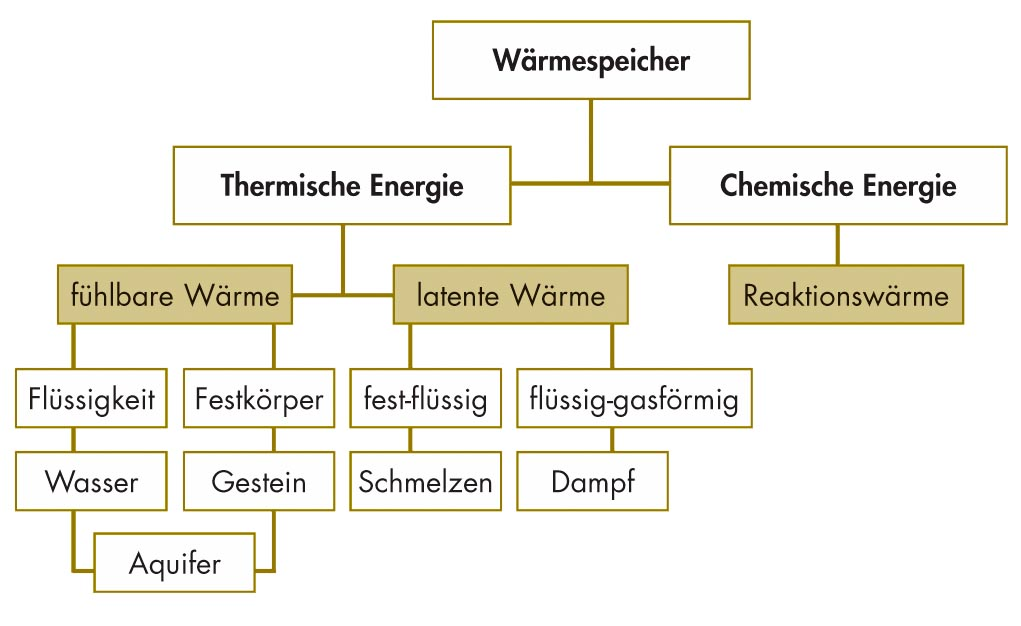
\includegraphics[scale=0.3]{images/speicher.jpg}
\caption{Übersicht über die verschiedenen Wärmespeichertechnolgien \cite{BINE}}
\label{fig:Wärmespeicher}
\end{center}
\end{figure}

\subsection{Chemische Speicher}
Chemische Speicher werden über eine chemsiche Reaktion be- und entladen. Per
Definition eines Speichers sind diese Reaktionen reversibel. Die nutzbare
Wärmeenergie entspricht der freigesetzten Reaktionsenthalpie $\Delta
H_{\mathrm{R}}$.
\section{Technologischer Überblick}
\subsection{Latentspeicher}
\subsubsection{Stand der Technik}
\subsubsection{Entwicklung}
\subsubsection{Perspektiven}
\subsubsection{Chancen}
\subsubsection{Herausforderungen}
\subsection{chemische Speicher}
\subsubsection{Stand der Technik}
\subsubsection{Entwicklung}
\subsubsection{Perspektiven}
\subsubsection{Chancen}
\subsubsection{Herausforderungen}


\newpage
\section{Einsatzgebiete}
\subsection{Latentwärmespeicher}
\subsection{chemische Speicher}

\newpage
\section{Ausblick}

\listoftables
\newpage
\listoffigures
\newpage
\begin{thebibliography}{99}
	\bibitem{BINE}BINE Energieforschung für die Praxis. Abgerufen am 11.04.2014 von
	http://www.bine.info/typo3temp/pics/b193b0972c.gif verändert durch D. Strebel
\end{thebibliography}
\end{document}
